\documentclass{article}
\usepackage{spalign}
\usepackage{graphicx}
\usepackage{amsmath}
\usepackage{amsfonts}
\usepackage{xcolor}

\title{Introduction to Limits \\ Notes}
\author{John Guzauckas}
\date{\today}

\begin{document}
\maketitle

\section{Objectives}
At the end of this sequence, and after some practice, you should be able to:
\begin{itemize}
    \item Use a calculator to determine right and left hand limits.
    \item Identify right and left hand limits based on graphs.
    \item Determine if a limit exists based on values of right and left hand limits.
    \item Understand that the limit does not depend on the value of a function at the point of interest.
\end{itemize}

\pagebreak
\section{Moving Closer and Closer}
Calculus is all about functions.
\\You probably know that a function $f$ takes an input $x$ and gives an output $f(x)$, which we could write as
$x \mapsto f(x)$.
\\But in calculus, we aren't concerned with just a single input and it's output, we want to consider
a whole range of inputs. We want to know what happens as the input moves/varies.
\\An example: As $x$ moves closer to $1$ from the left: $x \rightarrow 1^{-}$
\begin{center}
    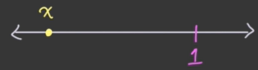
\includegraphics[scale = 1]{Images/MovingCloser1.png}
    \\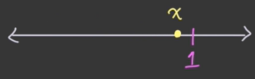
\includegraphics[scale = 1.01]{Images/MovingCloser2.png}        
\end{center}
It is important to note that when we say $x$ moves closer to $1$, we do not mean that $x$ will ever
equal $1$, we are only concerned with values of $x$ that are near $1$.
\\In a function $f$, we know that as we change our input $x$, our output $f(x)$ is going to change as well.
\\With limits, we ask the question, does the output $f(x)$ move close to something as the input $x$
moves close to something?
\\For our example, lets take the function $\frac{\sqrt{3 - 5x + x^{2} + x^{3}}}{x - 1}$.
\\To do this, we could take values for $x$ that are getting closer to $1$ from the left to use as
inputs for $f$.
\\There are an infinite amount of values we could choose for $x$, but we will start with 4 simpler values.
\begin{center}
    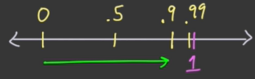
\includegraphics[scale = 1]{Images/MovingCloser3.png}\\
    \begin{tabular}{ c|c }
        $x$ & $f(x)$\\
        \hline
        $0$ & $f(0) \approx -1.73$\\
        $0.5$ & $f(0.5) \approx -1.87$\\
        $0.9$ & $f(0.9) \approx -1.97$\\
        $0.99$ & $f(0.99) \approx -1.997$
    \end{tabular}
\end{center}
Reading the values in this table, we can see that as $x$ approaches $1$ from the left, $f(x)$ approaches $-2$.
\\Now we can try to find what $f$ approaches as $x$ approaches $1$ from the right side.
\begin{center}
    \begin{tabular}{ c|c }
        $x$ & $f(x)$\\
        \hline
        $2$ & $f(2) \approx 2.23$\\
        $1.5$ & $f(1.5) \approx 2.12$\\
        $1.1$ & $f(1.1) \approx 2.02$\\
        $1.01$ & $f(1.01) \approx 2.003$
    \end{tabular}
\end{center}
This time, reading the values in the table, we can see that as $x$ approaches $1$ from the right, $f(x)$
approaches $2$.
\\That means that in this example, the direction we were approaching from with $x$ affected where
$f(x)$ was approaching.

\section{One-Sided Limits}
From the last section, we know that given the function $f(x) = \frac{\sqrt{3 - 5x + x^{2} + x^{3}}}{x - 1}$,
\begin{itemize}
    \item As $x \rightarrow 1^{-}$, $f(x) \rightarrow -2$
    \item As $x \rightarrow 1^{+}$, $f(x) \rightarrow 2$
\end{itemize}
We can plot the points we had in the tables from the last section on the coordinate plane to get a
better picture of what is happening with our function:
\begin{center}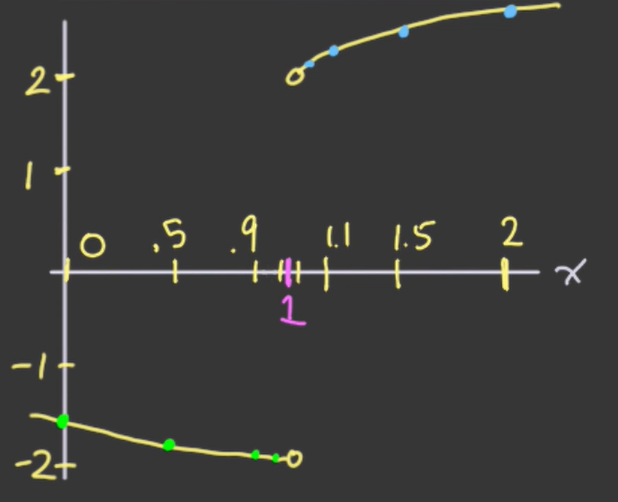
\includegraphics[scale = 0.5]{Images/OneSided1.png}\end{center}
We call this phenomena where a function approaches a value a \textbf{limit}
\\We could rephrase our earlier statements to use our new vocabulary and some new notation:
\begin{itemize}
    \item The limit of $f(x)$ as $x \rightarrow 1^{-}$ is $-2
        \Longrightarrow\underset{x \rightarrow 1^{-}}{\lim} f(x) = -2$
    \item The limit of $f(x)$ as $x \rightarrow 1^{+}$ is $2
        \Longrightarrow\underset{x \rightarrow 1^{+}}{\lim} f(x) = 2$
\end{itemize}
We call the limit as $x$ approaches a value from the left the \textbf{left-hand limit} and the limit
as $x$ approaches a value from the right the \textbf{right-hand limit}.

\end{document}